\section{Infrastructure}
Our infrastructure utilizes routers each installed with OpenWRT -- a free Linux-based router firmware -- running a cross-compiled version of tcpdump.  Specifically, our setup consisted of Buffalo AG300H routers, though any router with an omnidirectional antenna would serve adequately. The property that this infrastructure uses only free and open-source software and cheap, widely-available hardware differentiates it in the arenas of plausibility and realistic deployment from previous work that uses complicated, obscure, and/or special purpose (albeit possibly cheap) hardware. 

\begin{figure}[htb]
\begin{center}
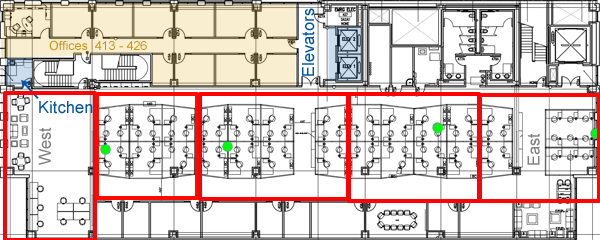
\includegraphics[width=\linewidth]{figs/floor4}
\end{center}
\caption{Location of routers (green) shown in relation to actuation zones (red). Note we do not need to place the routers in a convex hull of the entire floor in order to place a user within a zone.}
\end{figure}

The campus network on which we chose to deploy was a 2.4Ghz wireless network supporting channels 1, 6, and 11. Each of the routers was set to \emph{monitor/promiscuous} mode, and was installed with tcpdump-4.2.1, an open-source packet analyzer. Because routers typically lack the processing power and memory for processing large amounts of data, we connected our routers to a central computer (a FitPC running Ubuntu Linux). The manner of the connection between routers and central computer can be through a wired network or through direct Ethernet. It is the job of this central computer to mitigate the collection of packet data from each of the routers, perform the necessary mathematical operations, and process the results against a list of known MAC addresses. 

The routers cycle through each of the three wireless channels using tcpdump-4.2.1 to capture packets in 1-second increments. Each packet is forwarded along with its 802.11 radiotap link-level header over SSH to the central computer, which parses out the RSSI and source MAC address. For recognized MAC addresses, for each time-step for a given sample rate, each RSSI is converted to a linear scale and the resulting RSSIs are averaged per router. We can then compute the possible location $(x_d,y_d)$ of the device possessing a given MAC address as the centroid of the known router coordinates $(x_i, y_i)$ weighted by the average detected signal strength at that router $r_i$:
\begin{equation}
\begin{split}
x_d, y_d = \displaystyle\sum_{i} \frac{r_ix_i, r_iy_i}{\displaystyle\sum_i r_i}
\end{split}
\end{equation}
The central computer stores the 10 most recent computed centroids, and the location of the device is computed as the average of the 5 most closely clustered centroids of the 10 cached centroids (using Manhattan Distance as a heuristic). In practice, this ``averaging of averages'' greatly reduces the influence of the deployment environment upon the consistency of the measured RSSIs. Abnormally strong or weak signals thus do not alter the accuracy of our estimations. There is an incurred lag of about 4 times the sample rate should the device move, but this delay is acceptable within the bounds of accurate occupancy detection. We are able to place devices within 1 cubicle of their actual location (about 10 feet). This grade of accuracy is lower than other trained systems such as X Y and Z, but because light banks and HVAC dampers cannot differentiate between two adjacent cubicles, our system need not as well.

The passive nature of our localization infrastructure means that it requires little, if any, effort on behalf of the occupants to perform. It is only necessary for a device to associate with the available network before we can start tracking it. We can obtain a session IP address for a device with a given MAC address by listening to all wireless traffic. In the absence of regular or sufficient traffic, the central computer can occasionally ping the device in question to either elicit the requisite wireless traffic or determine if the device has left the tracking area (which suggests the user has left). This approach differs from previous wireless localization work in that it does not \emph{require} the user to ensure he/she is creating enough traffic to be localized accurately, but rather unobtrusively generates the necessary data. 

This raises the issue of accounting for ``detached devices,'' devices left connected to the network that are not actively being used and can therefore be falsely registered as occupants. This can be ignored in the context of binary occupancy detection (``occupied'' versus ``not occupied''), but in applications requiring more exact counts, the problem of detached devices can be approached with analysis of the specific types of packets sent by the device in question. For example, if the device is sending DHCP authentication packets, we can assume the device may have been associated with the given network for awhile but not logged-in, suggesting the device is not currently being used. Analysis of the number of HTTP packets for a given device can indicate the type and activity level of the device: low-frequency laptop traffic might suggest a detached device, whereas high-frequency mobile phone traffic implies an active user.

An additional strength of our infrastructure is the possibility for it to exist entirely on the incumbent router setup, e.g. by being installed as part of the proprietary Cisco router firmware. 

It is a simple matter to map arbitrary polygons to the areas affected by specific lightbanks or HVAC drivers, and thusly provide occupant-driven actuation. Systems such as BAS facilitate the actuation of a space based on geospatial coordinates.

In order to place an occupant within a space, it is necessary to have the routers form a convex hull of said space. However, because of the low granularity of building actuation controls, fewer routers may be used to 

\begin{figure}[htb]
\begin{center}
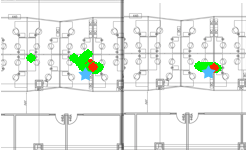
\includegraphics[width=.6\linewidth]{figs/samplesize}
\end{center}
\caption{increased accuracy with increasingly large sample rates (20s, left; 10s, right). Even at times of low ambient signal noise, weighted centroid measurements can be inconsistent (green), a problem remedied by averaging the 5 most closely clustered centroids (red).}
\end{figure}

\begin{itemize}
\item wireless localization tailored for buildings, passive is key. We reuse existing infrastructure (not entirely, actually, bec this is a prottype, but in real life we would get Cisco to do this on their routers)

\item need to elicit data from user phones

\item no need for training -- easily generalize

\item how easy this is to map into our current acutation setup

\item how is this better than existing solutions like RFID, motion sensors, laser gates, other wifi localization

\item include picture of setup of floor on SDH floor plan. Locations of routers, location of device, guessed centroids, 'averaged' centroids, etc

caption: increased accuracy with increasingly large sample rates. Even when measured at times of low ambient noise, measurements can be inconsistent (green/light grey), a problem remedied by averaging the 5 most closely clustered centroids (red/dark grey)

\item mac address and IPs, get traffic, pull out iP, generate traffic

\item how to detect stationary devices. We can do automatic detection, but if occupants abandon a device,  "detatched devices"

\end{itemize}